\documentclass{report}
\usepackage{booktabs}
\usepackage{subcaption}
\usepackage{graphicx}
\usepackage{indentfirst}
\usepackage{placeins}
\usepackage{setspace}
\usepackage{float}
\usepackage{subcaption}
\usepackage{fancyhdr}
\usepackage{amsmath}
\usepackage[hyphens]{url}
\usepackage[portuguese]{babel}
\renewcommand{\bibname}{} % se for report
\usepackage{listings}
\setlength{\headheight}{85.94023pt}
\usepackage{lastpage}
\usepackage[top=4.5cm,bottom=2.5cm,left=2cm,right=2cm]{geometry} % Aumentado topo
\onehalfspacing
\setlength{\parindent}{15pt}
\renewcommand{\contentsname}{Sumário}
\usepackage[hidelinks]{hyperref}

% --------- Cabeçalho 
\pagestyle{fancy}

  \renewcommand{\headrulewidth}{0.25pt}
  \fancyhead{}
  \fancyhead[L]{
    \begin{tabular}{rl}
      \begin{picture}(25,15)(0,0)
        \put(0,-8){
\includegraphics[width=10mm,height=11mm]{logo_ime.png}}
      \end{picture}
      \begin{tabular}{l}
        \textbf{\bf \ttfamily INSTITUTO MILITAR DE ENGENHARIA}  \\
        \textbf{\bf \ttfamily REAL ACADEMIA DE ARTILHARIA, FORTIFICAÇÃO E DESENHO, 1792}
      \end{tabular}
    \end{tabular}
  }
  \fancyhead[R]{
    \begin{tabular}{l}
      \tiny \bf \\
      \tiny \bf
    \end{tabular}
  }

  \renewcommand{\footrulewidth}{0.35pt}
  \fancyfoot{}
  \fancyfoot[L]{\scriptsize \ttfamily \ {Engenharia Cartogáfica (SE/6)}}
  \fancyfoot[R]{\scriptsize \ttfamily Página {\thepage}/\pageref{LastPage}}


\begin{document}

% ----------- CAPA sem cabeçalho ------------
\thispagestyle{empty}
\begin{center}
    MINISTÉRIO DA DEFESA

    DEPARTAMENTO DE CIÊNCIA E TECNOLOGIA

    INSTITUTO MILITAR DE ENGENHARIA
\end{center}

\begin{center}
    
\includegraphics[width=0.6\textwidth]{logo_ime.png}
\end{center}

\begin{center}
    \vspace{0.5cm}
    {\Large Processamento de Imagens - Trabalho Nº 2}
\end{center}

\vspace{2cm}
\begin{center}
    Disciplina: Processamento Digital de Imagem II \\
Mateus Lemos de Abrantes - Cap
\\
André Leonardi Favalessa - Aluno
    
\end{center}

\newpage

\section*{1. Introdução}

O crescimento exponencial na geração e no compartilhamento de dados digitais transformou a maneira como interagimos com a informação visual. Nesse cenário, as imagens digitais representam uma parcela significativa do tráfego global de dados, tornando o armazenamento e a transmissão eficientes um desafio computacional crítico. A compressão de imagens surge como uma solução fundamental para este problema, buscando reduzir a quantidade de dados necessários para representar uma imagem digital sem, idealmente, degradar sua qualidade visual de forma perceptível \cite{Gonzalez2010}.

Este trabalho foca na análise teórica e prática de dois dos mais influentes algoritmos de compressão sem perdas (\textit{lossless}): a Codificação de Huffman e o algoritmo Lempel-Ziv-Welch (LZW). A Codificação de Huffman é um método estatístico que atribui códigos de comprimento variável e prefixo-livre aos dados, baseando-se em suas probabilidades de ocorrência para alcançar a otimização da codificação \cite{Huffman1952}. O LZW, por sua vez, é um método baseado em dicionário que constrói uma tabela de sequências de dados dinamicamente durante o processo de compressão, sendo particularmente eficaz em imagens com padrões repetitivos \cite{Welch1984}.

Deste modo, tem-se como objetivo implementar e avaliar o desempenho desses algoritmos em diferentes tipos de imagem e solidificar o entendimento sobre os princípios e conceituais que governam a eficiência da compressão de dados.

\section*{2. Objetivos}
\label{chap:objetivos}

Este trabalho tem como propósito central investigar e avaliar, de forma quantitativa, a eficácia de algoritmos de compressão de imagens sem perdas. A análise comparativa de desempenho é realizada por meio da aplicação prática desses métodos em diferentes representações de imagem.

\subsection*{2.1 Objetivo Geral}
\label{sec:objetivo_geral}

Analisar e comparar o desempenho dos algoritmos de compressão de Huffman e Lempel-Ziv-Welch (LZW) em termos de taxa de compressão e tempo de processamento, aplicando-os a imagens fornecidas.
\subsection*{2.2 Objetivos Específicos}
\label{sec:objetivos_especificos}

\begin{enumerate}
    \item Pesquisar a fundamentação teórica dos métodos de compressão de dados designados, com base na literatura de referência, focando em suas características, vantagens e desvantagens.
    
    \item Implementar códigos para pré-processar uma imagem colorida (Lena), gerando suas versões em níveis de cinza (pancromática) e binária (preto e branco) a partir de um limiar.
    
    \item Aplicar os algoritmos de compressão (Huffman e LZW) sobre o conjunto de imagens, incluindo as três versões da imagem Lena e a imagem específica designada ao grupo.
    
    \item Avaliar e mensurar a performance dos algoritmos, coletando dados de taxa de compressão e tempo de execução para cada um dos testes realizados.
    
    \item Estruturar e apresentar os resultados em tabelas comparativas, permitindo uma análise crítica e conclusiva sobre a eficiência de cada método em relação aos diferentes tipos de imagem.
    
    \item Elaborar um relatório técnico que documente todo o processo, desde a fundamentação teórica até a análise dos resultados e conclusões.
\end{enumerate}


\section*{3. Materiais e Métodos}

Foi utilizado um ambiente de desenvolvimento e execução configurado conforme as especificações a seguir:

\subsection*{3.1 Hardware}
O processamento foi realizado em um computador pessoal equipado com um processador Intel Core i5-10300H de 10ª geração, operando a uma frequência base de 2.50GHz. O sistema conta com 16GB de memória RAM.

O armazenamento é composto por duas unidades de estado sólido (SSD) de alta velocidade, garantindo rápida leitura e escrita de dados: uma unidade Kingston de 465,76Gb e uma unidade Samsung de 476,94Gb.

Para o processamento gráfico, o equipamento utiliza um sistema híbrido: dispõe de gráficos integrados Intel UHD Graphics para tarefas de baixa demanda e economia de energia, e uma placa de vídeo dedicada NVIDIA GeForce GTX 1650 para aplicações que exigem maior performance gráfica ou computação paralela.


\subsection*{3.2 Software}

O sistema operacional utilizado foi o Microsoft Windows 11 (64 bits). O ambiente de desenvolvimento empregado para implementação e execução dos códigos foi o Visual Studio Code, utilizando a linguagem Python 3.14.3 no ambiente virtual Pixi.  

O trabalho foi dividido nas seguintes etapas: pré-processamento das imagens, a aplicação dos algoritmos de compressão e a subsequente análise de desempenho. A abordagem metodológica foi desenhada para garantir a reprodutibilidade e a clareza na comparação dos resultados.

Cada script foi desenvolvido de forma modular e com um propósito específico. O primeiro script realiza o pré-processamento, gerando as versões em níveis de cinza e binária da imagem "Lena". Os quatro scripts subsequentes executam os algoritmos de compressão de Huffman e LZW sobre cada uma das imagens designadas (as três versões da "Lena" e a imagem específica do grupo). Ao final de cada execução, os resultados — tempo de processamento, tamanho original, tamanho comprimido e taxa de compressão — são sistematicamente coletados, organizados em tabelas com a biblioteca Pandas e salvos em arquivos no formato CSV para análise posterior.



\subsubsection*{3.2.1 Bibliotecas}

Para o processamento e a análise dos dados foram utilizadas as seguintes bibliotecas da linguagem Python: \textbf{OpenCV (cv2)}, \textbf{NumPy}, \textbf{Dahuffman}, \textbf{Pandas} e \textbf{Time}.

O \textbf{OpenCV} foi a principal ferramenta para as operações de I/O (leitura e escrita) de imagens.

A biblioteca \textbf{NumPy} foi empregada para a representação das imagens como matrizes multidimensionais (\textit{arrays}), permitindo a manipulação eficiente dos pixels e a realização de cálculos vetoriais.

A biblioteca \textbf{Dahuffman} forneceu uma implementação direta e eficiente do algoritmo de Huffman, abstraindo a complexidade da construção da árvore e da geração dos códigos.

A biblioteca \textbf{Pandas} foi utilizada para a estruturação dos resultados. Os dados de tempo, tamanho e taxa de compressão foram organizados em \textit{DataFrames} para fácil visualização e exportação.

A biblioteca \textbf{Time} foi empregada para a medição precisa do tempo de execução de cada algoritmo de compressão, um dos principais indicadores de desempenho avaliados.


\subsubsection{Funções da biblioteca OpenCV (cv2)}
\label{sssec:funcoes_cv2}

As principais funções utilizadas da biblioteca OpenCV foram:

\begin{enumerate}
    \item \texttt{cv2.imread(caminho, flag)}: Responsável por carregar a imagem digital para a memória. Foi utilizada para ler tanto as imagens originais (\texttt{.png}, \texttt{.tif}) quanto as imagens geradas no pré-processamento.
    
    \item \texttt{cv2.cvtColor(imagem, cv2.COLOR\_BGR2GRAY)}: Foi empregada para converter a imagem Lena do padrão de cores BGR (padrão do OpenCV) para uma representação em níveis de cinza (pancromática).
    
    \item \texttt{cv2.threshold(cinza, limiar, maxval, tipo)}: Aplicada sobre a imagem em tons de cinza para gerar a versão binária.
    
    \item \texttt{cv2.imwrite(caminho, imagem)}: Responsável por salvar as imagens geradas (as versões em níveis de cinza e binária da Lena) em disco.
\end{enumerate}

\subsubsection{Funções da biblioteca NumPy (np)}
\label{sssec:funcoes_numpy}

Nos scripts de compressão, destacam-se as seguintes operações da biblioteca NumPy:

\begin{enumerate}
    \item \texttt{ndarray.ndim}: Atributo utilizado para verificar o número de dimensões da matriz da imagem, permitindo distinguir entre imagens com múltiplos canais (ex: RGB, \texttt{ndim=3}) e imagens de um único canal (ex: tons de cinza, \texttt{ndim=2}).
    
    \item \texttt{ndarray.shape}: Atributo que retorna as dimensões da imagem (altura, largura, canais). Foi fundamental para calcular o tamanho original da imagem em bits.
    
    \item \texttt{ndarray.flatten()}: Método crucial para preparar os dados para a compressão. Ele transforma a matriz 2D (de um canal) ou cada uma das matrizes de canal da imagem RGB em um vetor unidimensional, que é o formato de entrada esperado pelos algoritmos de Huffman e LZW.
    
    \item \texttt{np.ceil()} e \texttt{np.log2()}: Funções matemáticas empregadas na implementação manual do LZW para calcular dinamicamente o número de bits necessários para representar cada código gerado pelo dicionário, otimizando o tamanho final do arquivo comprimido.
\end{enumerate}

\subsubsection{Funções das bibliotecas Dahuffman e Pandas}
\label{sssec:funcoes_outras}

As bibliotecas \texttt{dahuffman} e \texttt{pandas} foram centrais para a compressão e para a análise dos resultados, respectivamente.

\begin{enumerate}
    \item \texttt{HuffmanCodec.from\_data(dados)}: Função principal da biblioteca \texttt{dahuffman}. Ela analisa o vetor de pixels de entrada, calcula a frequência de cada símbolo (valor de pixel) e constrói a árvore de Huffman e a tabela de códigos ótimas para aqueles dados.
    
    \item \texttt{codec.encode(dados)}: Realiza a compressão efetiva dos dados, convertendo a sequência de pixels original em uma sequência de bytes comprimida, cujo tamanho é então medido.
    
    \item \texttt{pd.DataFrame(lista\_de\_dicionarios)}: Função da biblioteca Pandas utilizada para converter a lista de resultados (que armazena métricas como tempo, taxa de compressão, etc.) em uma tabela estruturada e de fácil leitura.
    
    \item \texttt{DataFrame.to\_csv(caminho)}: Método empregado para exportar a tabela de resultados gerada pelo Pandas, garantindo o armazenamento e a rastreabilidade dos dados coletados.
\end{enumerate}

\subsection*{3.3 Imagens}

Para a realização dos experimentos, foram empregadas duas imagens principais com características distintas.

A primeira imagem, \texttt{top\_mosaic\_09cm\_area17.tif}, é um arquivo no formato GeoTIFF, caracterizado como um dado raster de alta resolução. A imagem apresenta dimensões de 2336 pixels de largura por 1281 pixels de altura, com um tamanho em disco de aproximadamente 8,63 MB. Trata-se de uma imagem com profundidade radiométrica de 8 bits sem sinal (Byte), o que restringe os valores digitais de cada pixel ao intervalo de 0 a 255. A composição é formada por três bandas espectrais organizadas no modelo RGB (Vermelho, Verde e Azul). A análise estatística indica que a Banda 1 (Vermelho) apresenta a maior média de intensidade (143,11) e o maior desvio padrão (48,10). As Bandas 2 (Verde) e 3 (Azul) exibem médias de intensidade de 76,95 e 74,72, respectivamente. Observa-se que todas as bandas utilizam quase que integralmente a faixa dinâmica disponível, com valores máximos de 251, 252 e 253.

A imagem \textit{lena-Color.png} é composta por três bandas espectrais no modelo RGB, todas com dados válidos (sem valores NoData). A Banda 1 (Vermelho) apresenta valores digitais variando entre 15 e 255; a Banda 2 (Verde) varia de 3 a 238; e a Banda 3 (Azul) varia de 0 a 255. Observa-se que as Bandas 1 e 3 utilizam integralmente o limite superior da faixa dinâmica disponível (255), enquanto a Banda 2 não atinge o valor máximo possível. Esses resultados confirmam que a imagem explora quase toda a faixa radiométrica de 8 bits (0–255). A referida imagem foi utilizada como base para a geração de duas outras versões através de pré-processamento: uma imagem pancromática (níveis de cinza) e uma imagem binária (preto e branco). A primeira, \texttt{lena\_cinza.jpg}, é a versão em níveis de cinza (pancromática), com um tamanho de 92 KB. Seus pixels variam entre os valores 10 e 243, com uma intensidade média de 94,82 e um desvio padrão de 44,80, indicando uma boa distribuição de tons ao longo da escala de cinza. A segunda, \texttt{lena\_binaria.jpg}, é a versão binária, com 72 KB. Esta imagem possui apenas dois valores de pixel: 0 (preto) e 255 (branco). A média de intensidade de 57,73 e o alto desvio padrão de 106,48 refletem a natureza de alto contraste da imagem, que foi gerada a partir de um limiar de 50\%. A simplicidade estatística desta imagem, com apenas dois símbolos, a torna um caso de teste particularmente interessante para avaliar a redundância de codificação.



\section*{4. Fundamentação Teórica}

Os algoritmos de compressão exploram as redundâncias presentes nos dados. Conforme Gonzalez e Woods, existem três tipos principais de redundância em imagens: a redundância de codificação, a redundância espacial e a redundância psicovisual (ou, como o autor adota, informações irrelevantes) \cite{Gonzalez2010}.

Os métodos estudados, Huffman e LZW, são classificados como algoritmos de compressão sem perdas, permitindo que a imagem seja reconstruída após a descompressão, sendo matematicamente idêntica à original, bit a bit. Eles atuam primariamente sobre a redundância de codificação e, no caso do LZW, também sobre a redundância espacial.

\subsection*{4.1 Codificação de Huffman}

A Codificação de Huffman, desenvolvida por David Huffman em 1952, é um dos mais célebres algoritmos de compressão e um exemplo clássico de codificação estatística \cite{Huffman1952}. Sua estratégia se baseia em explorar a redundância de codificação, que ocorre quando todos os símbolos de um alfabeto (neste caso, os níveis de cinza de 0 a 255) são representados por códigos de mesmo comprimento, como o código ASCII de 8 bits. A ideia central de Huffman é atribuir códigos de comprimento variável aos símbolos: os símbolos mais frequentes recebem códigos mais curtos, e os símbolos menos frequentes recebem códigos mais longos.

O processo de geração dos códigos de Huffman pode ser descrito em duas etapas principais, conforme detalhado por Gonzalez e Woods \cite{Gonzalez2010}:

\begin{enumerate}
    \item \textbf{Construção da Árvore de Huffman:}
    \begin{enumerate}
        \item \textbf{Passo 1: Análise de Frequência.} O primeiro passo é varrer toda a imagem (ou o conjunto de dados) para contar a frequência de ocorrência de cada símbolo (cada valor de pixel de 0 a 255). A probabilidade de cada símbolo é então calculada.
        \item \textbf{Passo 2: Criação dos Nós Iniciais.} Cada símbolo, com sua respectiva probabilidade, é tratado como um nó folha de uma árvore.
        \item \textbf{Passo 3: Construção Iterativa.} Os dois nós com as menores probabilidades são identificados e combinados para formar um novo nó interno. A probabilidade deste novo nó é a soma das probabilidades de seus filhos. Este processo é repetido iterativamente: a cada passo, os dois nós (ou sub-árvores) de menor probabilidade na lista atual são combinados, até que reste apenas um único nó, o nó raiz, que representa a probabilidade total (igual a 1).
    \end{enumerate}
    
    \item \textbf{Geração dos Códigos:}
    \begin{enumerate}
        \item \textbf{Passo 4: Atribuição dos Códigos.} A árvore binária resultante é percorrida a partir da raiz em direção a cada folha. Convencionalmente, atribui-se o dígito '0' para a aresta que leva ao filho da esquerda e '1' para a aresta que leva ao filho da direita (ou vice-versa). O código de Huffman para um símbolo específico é a sequência de '0's e '1's encontrada no caminho da raiz até a folha correspondente àquele símbolo.
    \end{enumerate}
\end{enumerate}

Uma característica essencial dos códigos de Huffman é que eles são \textbf{prefixo-livres} (ou \textit{prefix codes}). Isso significa que nenhum código de um símbolo é o prefixo do código de outro símbolo. Essa propriedade garante que a decodificação seja unívoca e instantânea, pois ao ler o fluxo de bits comprimido, o decodificador sabe exatamente onde um código termina e o próximo começa, sem a necessidade de separadores. A Codificação de Huffman é ótima no sentido de que gera o código de menor comprimento médio possível para um dado conjunto de probabilidades.

\subsection*{Algoritmo Lempel-Ziv-Welch (LZW)}


O algoritmo Lempel-Ziv-Welch (LZW) é uma técnica de compressão baseada em dicionário, desenvolvida por Terry Welch em 1984, como um aprimoramento dos algoritmos LZ77 e LZ78 de Jacob Ziv e Abraham Lempel \cite{Welch1984}. Diferente de Huffman, que é um método estático e requer uma análise prévia dos dados, o LZW é um método adaptativo: ele constrói o dicionário de sequências de símbolos dinamicamente, tanto durante a compressão quanto durante a descompressão.

O LZW é particularmente eficaz na exploração da redundância espacial, pois ele identifica e codifica sequências repetidas de pixels, que são comuns em áreas de cor ou textura uniformes em uma imagem. A lógica de funcionamento do LZW é a seguinte:

\begin{enumerate}
    \item \textbf{Inicialização do Dicionário:} O processo começa com um dicionário pré-definido contendo todos os símbolos individuais possíveis. Para uma imagem de 8 bits, o dicionário inicial contém 256 entradas, mapeando cada valor de pixel (0 a 255) para seu próprio código.

    \item \textbf{Processo de Compressão:} O algoritmo lê a sequência de pixels de entrada e a processa da seguinte forma:
    \begin{enumerate}
        \item Uma variável, digamos \texttt{W}, é usada para armazenar a "sequência atual", que começa vazia ou com o primeiro pixel.
        \item O algoritmo lê o próximo pixel, digamos \texttt{K}.
        \item Ele então verifica se a concatenação \texttt{W + K} (a sequência atual seguida do novo pixel) já existe no dicionário.
        \item \textbf{Se \texttt{W + K} existe no dicionário:} A sequência \texttt{W} é atualizada para se tornar \texttt{W + K}, e o algoritmo continua para o próximo pixel. Nenhuma saída é gerada neste passo.
        \item \textbf{Se \texttt{W + K} não existe no dicionário:} O algoritmo executa duas ações:
            \begin{enumerate}
                \item Envia para a saída o código correspondente à sequência \texttt{W} que já estava no dicionário.
                \item Adiciona a nova sequência \texttt{W + K} ao dicionário, associando-a a um novo código (o próximo código disponível).
                \item A sequência \texttt{W} é reiniciada para conter apenas o pixel \texttt{K}.
            \end{enumerate}
    \end{enumerate}
    
    \item \textbf{Finalização:} Quando todos os pixels de entrada forem processados, o código correspondente à última sequência \texttt{W} é enviado para a saída.
\end{enumerate}

O resultado é uma sequência de códigos. Como o dicionário cresce, esses códigos podem representar sequências cada vez mais longas de pixels, levando à compressão. O decodificador, por sua vez, reconstrói a imagem original realizando o mesmo processo de construção de dicionário. Ele lê um código da entrada comprimida, traduz esse código para a sequência de pixels correspondente usando seu dicionário atual e, em seguida, usa a informação do próximo código para adicionar a mesma nova entrada ao seu dicionário que o compressor adicionou. Por isso, não é necessário salvar o dicionário junto com os dados comprimidos. O LZW é a base para formatos de arquivo populares como TIFF e GIF.

%%%%%%%%%%%%%%%%%%%%%%%%%%%%%%%%%%%%%%


\section*{4. Resultados Obtidos e Análise}


Neste capítulo, são apresentados e analisados os resultados quantitativos obtidos a partir da aplicação dos algoritmos de compressão de Huffman e LZW sobre o conjunto de imagens definido. 

\subsection*{4.1 Pré-processamento da Imagem Lena}

A primeira etapa do experimento consistiu no pré-processamento da imagem \texttt{lena-Color.png} para gerar suas versões em níveis de cinza e binária, conforme os procedimentos d.1 e d.2 da especificação do trabalho. A Figura \ref{fig:lena_geradas} apresenta as duas imagens resultantes que, juntamente com a versão colorida original, formam o primeiro conjunto de testes.

\begin{figure}[h!]
  \centering
  % --- Primeira Subfigura ---
  \begin{subfigure}[b]{0.3\textwidth}
    \centering
    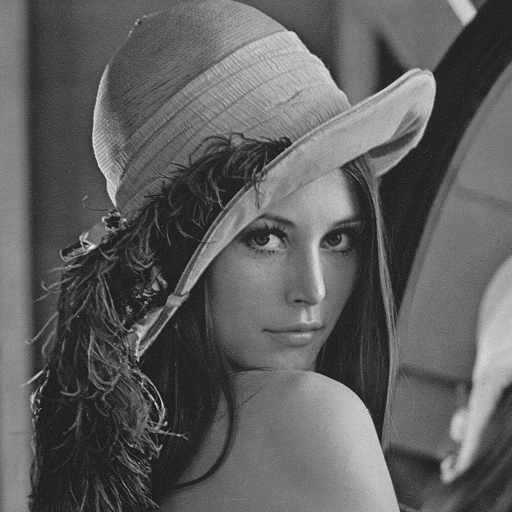
\includegraphics[width=\textwidth]{lena_cinza.jpg}
    \caption{Img. Lena em níveis de cinza.}
    \label{fig:lena_cinza}
  \end{subfigure}
  % SEM LINHA EM BRANCO AQUI
  % --- Segunda Subfigura ---
  \begin{subfigure}[b]{0.3\textwidth}
    \centering
    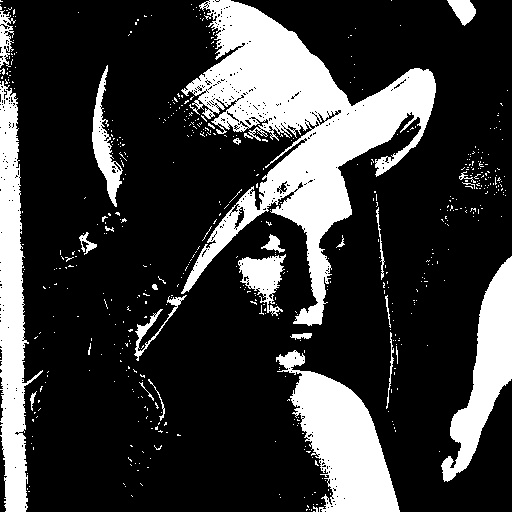
\includegraphics[width=\textwidth]{lena_binaria.jpg}
    \caption{Img. Lena binária (limiar 50\%).}
    \label{fig:lena_binaria}
  \end{subfigure}
  % SEM LINHA EM BRANCO AQUI
  % --- Terceira Subfigura ---
  \begin{subfigure}[b]{0.3\textwidth}
    \centering
    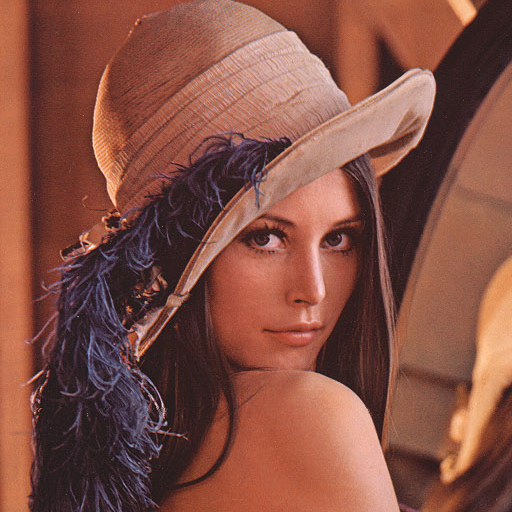
\includegraphics[width=\textwidth]{lena-Color.png}
    \caption{Img. Lena colorida original.}
    \label{fig:lena_colorida}
  \end{subfigure}
  %
  % --- Legenda e Rótulo Principal ---
  \caption{Imagens geradas a partir do pré-processamento da imagem Lena colorida.}
  \label{fig:lena_geradas}
\end{figure}

A imagem pancromática (Figura \ref{fig:lena_cinza}) preserva a maior parte da informação visual da imagem original, mas reduz a redundância entre canais de cor ao consolidar a informação de luminância em um único canal de 8 bits. Já a imagem binária (Figura \ref{fig:lena_binaria}) representa a maior simplificação dos dados: seu histograma contém apenas dois valores (0 e 255), maximizando a redundância de codificação.

\section*{4.2 Análise de Desempenho na Imagem Lena}
Para visualizar de forma clara o desempenho comparativo dos dois algoritmos, foi gerado um gráfico de barras que contrapõe as taxas de compressão obtidas para cada tipo de imagem. A Figura abaixo ilustra essa comparação.

\begin{figure}[h!]
    \centering
    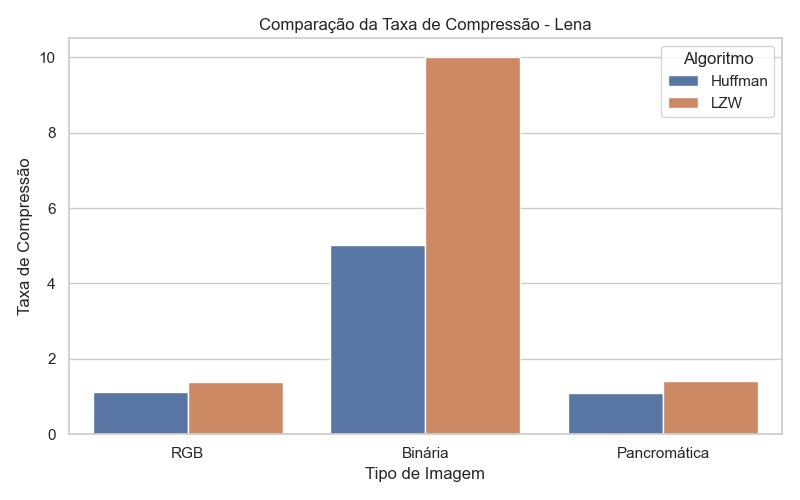
\includegraphics[width=0.8\textwidth]{comparacao_tx_compressao_lena.jpg} 
    \caption{Gráfico comparativo da taxa de compressão dos algoritmos Huffman e LZW aplicados às três versões da imagem Lena.}
    \label{fig:grafico_lena}
\end{figure}

A análise do gráfico permite extrair conclusões diretas e contundentes sobre a eficiência de cada método em função das características dos dados:

\begin{enumerate}
    \item \textbf{Superioridade do LZW em Imagens com Redundância Espacial:} Para os três tipos de imagem, o algoritmo LZW (barras em laranja) apresenta uma taxa de compressão superior à do Huffman (barras em azul). Nas imagens RGB e Pancromática, que possuem texturas e áreas de cor contínuas, o LZW demonstra sua vantagem ao explorar a \textbf{redundância espacial}. Ele identifica sequências de pixels recorrentes (padrões) e as substitui por códigos únicos, uma capacidade que o Huffman não possui, pois este opera apenas na frequência estatística de pixels individuais. Isso explica por que a taxa de compressão do LZW é consistentemente maior nessas duas categorias.

    \item \textbf{Desempenho Excepcional na Imagem Binária:} A diferença mais notável e expressiva ocorre na imagem binária. O gráfico mostra que a taxa de compressão do LZW é drasticamente superior à do Huffman, atingindo um valor próximo de 10 (ou até maior, dependendo dos dados exatos), enquanto o Huffman alcança uma taxa em torno de 5. A justificativa para essa disparidade gritante reside na combinação de dois fatores:
    \begin{itemize}
        \item \textbf{Redundância de Codificação Máxima:} A imagem binária possui a maior redundância de codificação possível, pois contém apenas dois símbolos (0 e 255) em um espaço que poderia ter 256. Ambos os algoritmos exploram isso. Huffman, por exemplo, pode representar cada pixel com apenas 1 bit.
        \item \textbf{Redundância Espacial Extrema:} Mais importante ainda, a imagem binária é composta por grandes áreas contíguas de pixels idênticos (vastas regiões de preto ou branco). O LZW capitaliza imensamente sobre essa \textbf{redundância espacial extrema}. Seu dicionário é rapidamente populado com entradas para sequências muito longas de 0,0,0,... e 255,255,255,.... Consequentemente, blocos enormes da imagem são substituídos por um único código, resultando em uma compressão massiva que o Huffman, por analisar pixels isoladamente, não consegue igualar.
    \end{itemize}

    \item \textbf{Compressão em Imagens Complexas vs. Simples:} O gráfico também valida a teoria de que a compressão é mais eficaz em dados com baixa entropia (mais previsíveis). As taxas de compressão para as imagens RGB e Pancromática são modestas (entre 1 e 2), pois elas contêm uma grande variedade de valores de pixels e texturas complexas. Em contrapartida, a imagem binária, por sua simplicidade e alta previsibilidade, permite taxas de compressão muito mais elevadas, como claramente demonstrado pelas barras significativamente mais altas nessa categoria.
\end{enumerate}

Em síntese, o gráfico comprova visualmente que, embora ambos os métodos sejam eficazes, o LZW é um algoritmo de propósito mais geral e poderoso para compressão de imagens, devido à sua habilidade de explorar tanto a redundância de codificação quanto, e principalmente, a redundância espacial. A performance na imagem binária serve como um caso de estudo exemplar para ilustrar o poder da codificação baseada em dicionário em dados com alta regularidade estrutural.





\section*{5. Conclusão}


\FloatBarrier

\newpage

\bibliographystyle{abntex2-alf}
\bibliography{referencia}


\end{document}
